\section{Datasets}\label{datasets}
\paragraph{MS-COCO}\cite{linMicrosoftCOCOCommon2015}
The MS-COCO dataset comprises images of everyday scenes with common objects to advance object 
recognition within the context of scene understanding. 
There are 82,783 training, 40,504 validation, and 40,775 testing images, 
all of which contain 80 common object categories. 
This dataset is commonly used for state-of-the-art benchmarking in object recognition and 
classification including multi-label classification.

\begin{figure}[h!]
\centering
\begin{subfigure}[b]{0.4\linewidth}
    
\includegraphics[width=0.8\linewidth]{fig/COCO_example.png}
\end{subfigure}
\begin{subfigure}[b]{0.4\linewidth}
    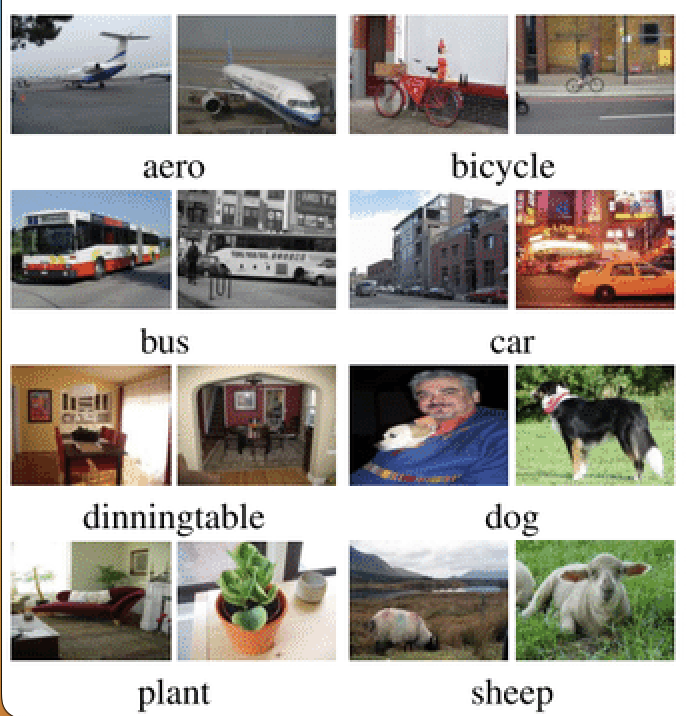
\includegraphics[width=1.3\linewidth]{fig/Pascal_example.png}
\end{subfigure}
\caption{Examples of images from dataset MS-COCO and Pascal-VOC. MS-COCO: Picture containing objects from categories `person', `tie', `bowl', `chair', `dining table' and `clock'.}
\label{fig:coco_pascal}
\end{figure}

\paragraph{VOC-Pascal}\cite{everinghamPascalVisualObject2015}
It is good for multi-label classification because it includes a variety of object categories, allowing for the evaluation of algorithms that can recognize and detect multiple objects in an image. 
PASCAL-VOC has 22,531 images, which are divided into 20 classes.

\paragraph{ImageNet}\cite{dengImageNetLargescaleHierarchical2009}
ImageNet is a large-scale hierarchical image database built upon the WordNet structure. 
Compared to small image datasets like Caltech101/256, MSRC, and PASCAL, ImageNet is much larger in scale and diversity, 
offering 20× the number of categories and 100× the number of total images.
ImageNet is often use not only for benchmarking for the variety of image but also for pre-trained models.

\begin{figure}[h!]
\centering
\begin{subfigure}[b]{0.4\linewidth}
    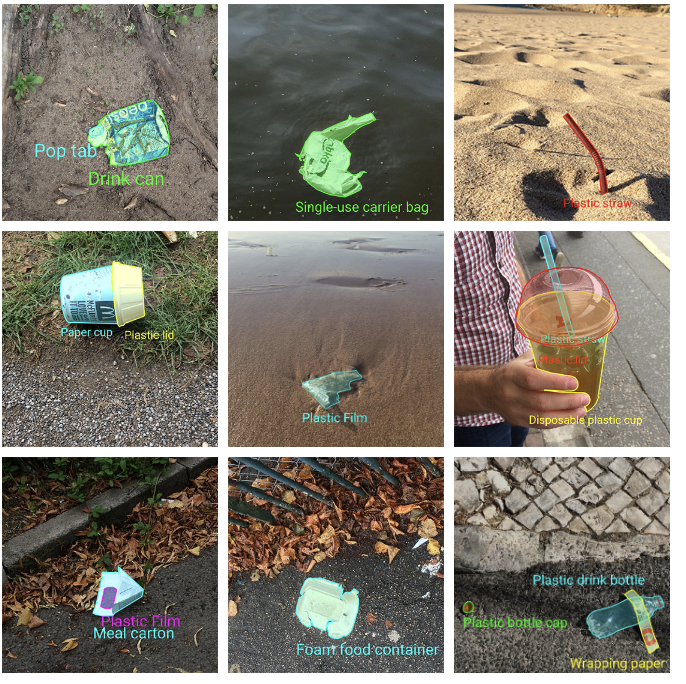
\includegraphics[width=\linewidth]{fig/TACO_example.png}
\end{subfigure}
\begin{subfigure}[b]{0.4\linewidth}
    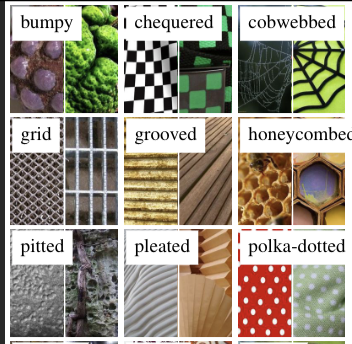
\includegraphics[width=1\linewidth]{fig/textures_example.png}
\end{subfigure}
\caption{Examples of images with label annotations from dataset TACO and Textures.}
\label{fig:coco_pascal}
\end{figure}

\paragraph{TACO}\cite{proencaTACOTrashAnnotations2020}
The TACO dataset is designed for litter detection and segmentation 
with 1500 high-resolution images and 4784 annotations. 
Litter detection is a challenging problem for multiple reasons so this dataset can be use to show the robustness of classifiers. 
